
\chapter{Propiedades generales de los núcleos}

% Buscar problema del signo (propiedades emergentgse)
% Explayarse bastante con el angulo solido (muy importnatne)

\section{Introducción: definiciones.}

\begin{definition}[\textbf{número atómico}]
	El número atómico (Z) de un núcleo es un entero que coincide con el número de protones del núcleo.
\end{definition}


\begin{definition}[\textbf{número másico}]
	El número másico (A) de un núcleo es la suma de número de protones y neutrones $A=Z+N$.
\end{definition}

Atendiendo a los valores $Z,A$ y $N$, los núcleos se clasifican en:

\begin{itemize}
	\item \textbf{Isótopos}: son núcleos con igual $Z$.
	\item \textbf{Isóbaros}: son núcleos con igual $A$.
	\item \textbf{Isotónos}: son núcleos con igual $N$.
\end{itemize}

Para denotar un núcleo se suele escribir $^A_Z X_N$ donde $X$ es el símbolo químico del elemento en cuestión (determinado por el valor $Z$). Protones y neutrones se denominan genéricamente \textbf{nucleones}. Hoy en día se han identificado alrededor de 112 átomos diferentes.

\subsection{Tipos de desintegraciones}

\subsubsection{Desintegración $\alpha$}

% hablar un poco de la distribución de poisson 

La desintegración alfa consiste en la emisión de dos protones y dos neutrones (un núcleo de helio) por parte de un núcleo inestable. Produce un desplazamiento hacia la izquierda de dos posiciones de la tabla periódica, y reduce el número másico en 4 unidades $\Delta Z = -2$ y $\Delta A  = -4$. Esquemáticamente esta desintegración se puede escribir Coulomb

\begin{equation}
	^A_Z X_N \longrightarrow ^{A-4}_{Z-2} Y_{N-2} + ^4_2\He_2
\end{equation}

Aunque en capítulos posteriores estudiaremos en detalle la evolución de las poblaciones de núcleos radioactivos, recordaremos ahora que la \textbf{vida media} ($\tau$) de un núcleo es el tiempo necesario para reducir el número de núcleos de una muestra en un factor $1/e$ de su valor inicial (o, en otras palabras, el promedio del tiempo que tarda un núcleo en desintegrarse), mientras que el período de semidesintegración ($t_{1/2}$) es el tiempo necesario para reducirlo a la mitad. Dados $N_0$ núcleos radioactivos iniciales qeu no están reponiéndose por medio de ningún proceso, el número de desintegraciones que se observan por unidad de tiempo es proporcional al propio númeo de núcleos presentes. La constante de proporcionalidad es característica de cada núcleo y se denomina \textbf{constante de desintegración} $\lambda$ que tiene unidades inversas de tiempo. Esto nos lleva a la ley de desintegración radiaciva:

\begin{equation}
	\frac{\D N}{\D t} = - \lambda N \Rightarrow N (t)  = N_0 e^{-\lambda t} \quad \tau = \frac{1}{\lambda}
\end{equation}
Otras definiciones de interés son el \textbf{semi tiempo}, esto es, el tiempo que tarda una muestra en reducirse a la mitad:

\begin{equation}
	t_{1/2} = \frac{\ln 2}{\lambda}
\end{equation}
La \textbf{actividad de una sustancia} se define como
\begin{equation}
	A(t)=\lambda N(t)  = A_0 e^{-\lambda t}
\end{equation}
y en el SI se define como Becquerelio (Bq, una desintegración en cada segundo). Para desarrollar estes conceptos véase el apartado \ref{Subsec:02-04-01}.

\subsubsection{Desintegración $\beta$}

La desintegración beta consiste en la conversión nuclear de neutrones en protones o viceversa. Por decirle de algún modo, es la manera en que el núcleo \textit{corrige} un exceso de protones o neutrones convirtiendo unos en otros. En física nuclear se suele usar los símbolos $\beta^-$ y $\beta^+$ para designar las radiaciones emitidas por las desintegraciones beta. La desintegración por emisión $\beta^-$ ($\beta^+)$ produce un desplazamiento hacia la derecha (izquierda) de una posible en la tabla periódica, pero no cambia esencialmente la masa: $\Delta Z = \pm, \Delta A = 0$. Responsable de este fenómeno es la intearcción débil:

\begin{equation}
	^A_Z X_N \longrightarrow ^A_{Z+1} Y_{N-1} + \beta^-
\end{equation}
\begin{equation}
	^A_Z X_N \longrightarrow ^A_{Z-1} Y_{N+1} + \beta^+
\end{equation}
La conversión nuclear en protones puede tener lugar de 3 modos distintos. En notación de física de partículas se escribe:

\begin{equation}
	n \longrightarrow p + e^- + \bar{\nu}_e  \tquad \text{desintegración} \ \beta^-
\end{equation}
\begin{equation}
	p \longrightarrow n + e^+ + {\nu}_e \tquad \text{desintegración} \ \beta^+
\end{equation}
\begin{equation}
	p + e^- \longrightarrow n + {\nu}_e \tquad \text{captura electrónica (CE} \ \epsilon)
\end{equation}
El tercer proceso un electrón de las capas internas (usualmente la K) con cierta probabilidad presencia dentro de la región nuclear es \textit{usado} para la consversión de un protón en un neutrón.

\subsubsection{Desintegración $\gamma$}

Los rayos $\gamma$ son capaces de penetrar varios milímetros en plomo. No son desviados por los campos electromangéticos e interaccionan con la materia de manera similar a los rayos X. Se trata de radiación electromagnética, e inicialmente se confundieron con los rayos X emitidos por el reordenamiento de los electrones atómicos que sigue a una conversión interna. La desintegración gamma consiste en la emisión espontánea de fotones altamente energétivcos cuando el núcleo pasa de un estado excitado a otro estado de menor energía o al fundamental. Es, por tanto, un proceso esencialmente análogo al que tiene lugar cuando un átomo se desexcita emitiendo radiación, bien sea en el rango visible o en el de rayos X. La emisión gamma suele acompañar a otros dos tipos de desintegración, porque sus procesos quedan normalmente en estados excitados.

\subsubsection{Fisión espontánea}

Es un proceso  en el que el núcleo pesado se divide en dos más ligeros. No es posible determinar a priori en qué par concreto de núcleos ligeros terminará, sino que habrá una distribución estadística en un cierto rango de números atómicos.

\subsubsection{Emisión nuclear}

Este es un proceso mediante el que un núcleo inestable, generalmente producto de una fisión o desintegración anterior, emite un nucleón.

\section{Masas de los núcleos}

En el laboratorio se miden masas atómicas, no masas nucleares. A pesar de ello, veremos que en casi todos los casos prácticos de la física nuclear podremos usar masas atómicas en lugar de masas nucleares, porque las masas de los electrones y sus energías de ligadura se cancelarán casi perfectamente en el balance global. Actualmente las masas atómicas se miden en unidades atómicas de masa unificadas (u), y se definen de manera que la masa del átomo $^{12}$C sea exactamente de 12u. La conversión de unidades:

\begin{equation}
	1u = 931.49432(28) \unit{\MeV/c^2} = 1.6605402(10) \times 10^{-27} \unit{\kg}
\end{equation}
Las masas del protón, neutrón y electrón:
\begin{equation}
	m_p = 939.272  \ \unit{\MeV/c^2} = 1836.149 \ m_e
\end{equation} 
\begin{equation}
	m_p = 939.565 \ \unit{\MeV/c^2} = 1838.679 \ m_e
\end{equation}
\begin{equation}
	m_e = 0.511 \ \unit{\MeV/c^2}
\end{equation}
Otra realación interesante

\begin{equation}
	c^2 = 931.494013(37)\ \unit{\MeV/u}
\end{equation}

\subsection{Espectrometría de masas}

Para medir las masas de isótopos radioactivos de vida media corta se recurre a las ecuaciones de balance energético en reacciones nucleares. En la reacción $x+X\rightarrow y+Y$, midiendo las energías cinéticas de cada compuesto para determinar la diferencia de masas, que se conoce como el \textbf{valor $Q$} de la reacción:

\begin{equation}
	Q=[m(x)+m(X)-m(y)-m(Y)]c^2 = E_c (\text{estado final}) -  E_c (\text{estado inicial})
\end{equation}
Donde la letra minúscula denota las masas nucleares. Para que una desintegración sea espontánea debe verificarse que $Q>0$, lo cual es evidnete, ya que la energía cinética del estado final no puede ser negativa, como por ejemplo en el caso de tener una sola partícula, podremos encontrar un sistema de referencia inercial donde esta partícula este en reposo, y por tanto $E_c (\text{estado inicial})=0$, de tal manera que si $Q<0$ implicaría $E_c (\text{final})<0$ lo cual no tiene sentido.

\subsection{Energía de ligadura}

Todo sistema compuesto (sistema ligado) tiene una energía de ligadura negativa, de tal manera que es energéticamente más favorable mantener unidos a los constituyentes que mantenerlos separados. En otras palabras: la suma de las masas de los contituyentes de un compeusto estable es mayor que la masa del compuesto. Esto es así porque existe una reacción de carácter atractivo entre los constituyentes que los mantiene unidos, de tal manera que es necesario realizar un trabajo para separlos y destruir (desintegrar) el compuesto. En el domino de la física nuclear definiremos la energía de un núcleo de modo que resulte positiva (masas de los constituyentes menos masa del compuesto).

La energía de la ligadura nuclear en términos de las masas atómicas de los elementos considerados que es lo que realmente se mide en el laboratorio. Para aclarar la notació, en lo que sigue usaremos la letra $m$ para representarla masa de una partícula, por ejemplo $m_n$ para la masa de un neutrón. Usaremos la notación $m(Z,A)$ para representar la \textbf{masa del núcleo} (\textbf{masa nuclear}), y la notación $M(Z,A)$ o $M(_Z^A X_N$) para designar la \textbf{masa de un átomo} (\textbf{masa atómica}) con $Z$ protones y $A$ nucleones. De esta manera podemos realcionar la masa atómica con la masa nuclear de la siguiente manera:

\begin{equation}
	M(Z,A) = m(Z,A)+ Zm_e - \frac{1}{c^2} \sum_{i=1}^Z B_i
\end{equation}
donde $B_i$ son las \textit{energía de ligadura} de los electrones. Este término es despreciable, por lo que la masa atómica y la masa nuclear se pueden relacionar por:

\begin{equation}
	M(Z,A) \approx m(Z,A) + Zm_e
\end{equation}
El valor de la masa nuclear también se puede expresar en función de la masas de sus constituyentes y la \textbf{energía de ligadura del núcleo} o \textbf{energía de ligadura nuclear} $B$:

\begin{equation}
	m(Z,A) =Zm_p + (A-Z)m_n - \frac{1}{c^2} B
\end{equation}
Es muy interesante expresar $B$ en función de parámetros conocidos, como son las masas atómicas y las masas de los protones, neutrones y electrones, ya que es la energía de ligadura la que nos va a permitir calcular si una desintegración podría ocurrir de manera espontánea o no. Así:

\begin{equation}
	\frac{1}{c^2} B = Zm_p + (A-Z)m_n - m(Z,A)
\end{equation}
en algunas de las tablas en lugar de tabular $M(Z,A)$ se proporciona el llamado \textbf{defecto de masa} $\Delta = (M-A)c^2$ donde $M$ es la masa atómica en \textit{uma} y $A$ es el número másico. Dado $\Delta$ se puede deducir la masa atómica.



\subsection{Formula semiempírica de masas}

Existe una fórmula que describe cualitativamente la energía de ligadura por nucleon. Se trata de \textbf{fórmula semiempírica de masas}, también conocida como \textbf{fórmula de Wizsäcker}, y es esencialmente una parametrización de la energía de ligadura aunque se la conoce como fórmula de masas porque la relación entre una y otra es directa. Esta parametrización se basa en el \textbf{modelo de la gota líquida}. Al igual que en una gota líquido, la densidad en el núcleo es esencialmente constante en función del radio nuclear:

\begin{equation}
	M(^A_ZX_N) \equiv M(Z,A) = ZM(^1 H) + Nm_n - \frac{B(Z,A)}{c^2}
\end{equation}
\begin{equation}
	B(Z,A) = a_v A - a_s A^{2/3} - a_c Z(Z-1) A^{-1/3} - a_{sy} \frac{(A-2Z)^2}{A} + \delta (A)
\end{equation}
Existen distintas parametrizaciones de la fórmula de masas, pero en todas ellas los términos son los mismos salvo constantes. Una breve descripción de cada uno de los términos es el siguiente:

\begin{itemize}
	\item \textbf{Término de volumen:} sabemos que la energía de ligdaura por nucleón es casi constante en función de $A$, esto es: $B\propto A$, luego el significado de $a_v A$ es obvio. $a_v$ será presumiblemente del orden de 8 MeV. Cada nucleón contribuye aproximadamente lo mismo a la energía de ligadura porque la interacción fuerte es de corto alcance y sólo le permite interaccionar con sus vecinos más próximos.
	\item \textbf{Término de superficie:} cerca de la superficie del núcleo es de esperar que los nucleones tengan menos vecinos y por lo tanto contribuyan un poco menos que los interiores a la energía de ligadura. El radio del núcleo va como $A^{1/3}$ y la superficie como $A^{2/3}$, por lo tanto el término de superficie es de la forma $a_s A^{2/3}$, contribuyendo con signo opuesto al de volumen para contrarrestar su excesivo peso.
	\item \textbf{Término de energía coulombiana:} la repulsión coulombiana entre los protones hace disminuir la energía de ligadura y, por lo tanto, aumentar la masa del núcleo. Debido al carácter de largo alcance de esta interacción, este término es proporcional a $Z^2$ e inversalemente proporcional al radio $a_c Z(Z-1)A^{-1/3}$ \footnote{Si realizaramos el cálculo suponiendo una esfera uniformemente cargada obtendríamos  una energía potencial dada por la expresión $-(3/5)e^2 Z^2 A^{-1/3}$. Si consideramos objetos puntuales uniformemente distribuidos en la \textit{esfera nuclear}, aparece en lugar de $Z^2$ el factor $Z(Z-1)$, proporcional al número de parejas de objetos: $-(3/5)e^2Z(Z-1)A^{-1/3} / (4\pi \epsilon_0 R_0)$. En la fórmula semiempírica de masas puede ser más conveniente dejar una constante global para ajustar los datos que usar un valor como $R_0=1.2$ fm en la expresión analítica anterior.}.
	\item \textbf{Término de simetría:} de la carta de Segré sabemos que la estabilidad nuclear se concreta en valores $Z\approx A/2$, y esto hemos de tenerlo en cuenta de alguna manera en nuestra fórmula de masas, de lo contrario no habría impedimento alguno para que la parametrización resultante no proporcionase isótopos estables con cientos de neutrones. Una posible forma de este parámetro es $-a_{sy} (A-2Z^2)/A$. Así escrito favorece la existencia de núcleos con un núemro parecido de protones y neutrones, y tiene mayor importancia para los núcleos ligeros, para los que la condición $Z\approx A/2$ es más estricta.
	\item \textbf{Término de pairing o apareamiento.} Un estudio significativo de las masas nucleares muestra que los nucleos más estables tienen un número par de protones y/o neutrones. Esto se debe a una tendencia de los nucleones a acoplarse en parejas de iguales, es decir pp y nn, con espines y momentos antiparalelos. Si tomtamos nulo este término ($\delta=0$) para núcleos con $A$ impar, entonces en núcleos con $Z$ impar y $N$ impar $\delta$ contribuye con signo negativo, es decir, tiende a disminuir la energía de ligadura y aumentar la masa del núcleo. Sería ventajoso en estos casos convertir uno de los protones en nuetrón o alguno de los neutrones en un protón. Finalmente, para núcleos con $Z$ par y $N$ par, $\delta$ contribuye con signo positivo. En la naturaleza sólo existen 4 núcleos impar-impar estables, que son el $^2$H, $^6$Li, $^{10}$B y $^{14}$ N, mientras que núcleos estables par-par hay unos 167, lo cual da una idea de la importancia del término pairing.
	      \begin{equation}
		      \delta (A) = \left\lbrace \begin{array}{rl}
			      +a_p A^{-3/4} & \text{Núcleos con Z par y N par}     \\
			      0             & \text{Núcleos con A impar}           \\
			      -a_p A^{-3/4} & \text{Núcleos con Z impar y N impar}
		      \end{array} \right \rbrace
	      \end{equation}
\end{itemize}
Las constantes se ajustan a los datos experimentales, con los siguientes valores como su mejor ajuste

\begin{table}[h!] \centering
	\begin{tabular}{ccccc}
		$a_v$ (MeV) & $a_s$ (MeV) & $a_c$ (MeV) & $a_{sy}$ (MeV) & $a_p$  (MeV) \\ \hline
		15.5        & 16.8        & 0.72        & 23             & 34
	\end{tabular}
\end{table}

\subsection{Aplicaciones de la formula semiempírica: parábola de masas}

La importancia de la fórmula de Weizsäcker no es que nos permita predecir nuevos fenómeno en física nuclear (que no lo hace), sino que representa un primer intento de modelizar el comportamiento de una propiedad nuclear como lo es la energía de ligadura. Contiene de hecho ingredientes de dos modelos nucleares: el modelo de la gota líquida y el modelo de capas. El primero trata alguna de las propiedades colectivas del núcleo de un modo similar a como se estudia en una pequeña gota líquida; los tres primeros términos de la energía de ligadura de la fórmula de Weizsäcker también aparecerían en el cálculo de la energía de ligadura que aparece en el modelo de una fota cargada. El modelo de capas contempla los nucleones desde una perspectiva individual y sería el contexto para la explicación de los dos últimos términos. Definimos el \textbf{exceso de masas} de un nucleido $\Delta(Z,A)$ como la diferencia entre su masa real y su número másico

\begin{equation}
	\Delta(Z,A) = M(Z,A) - (Z+N)m_u
\end{equation}

\begin{figure}[h!] \centering
	 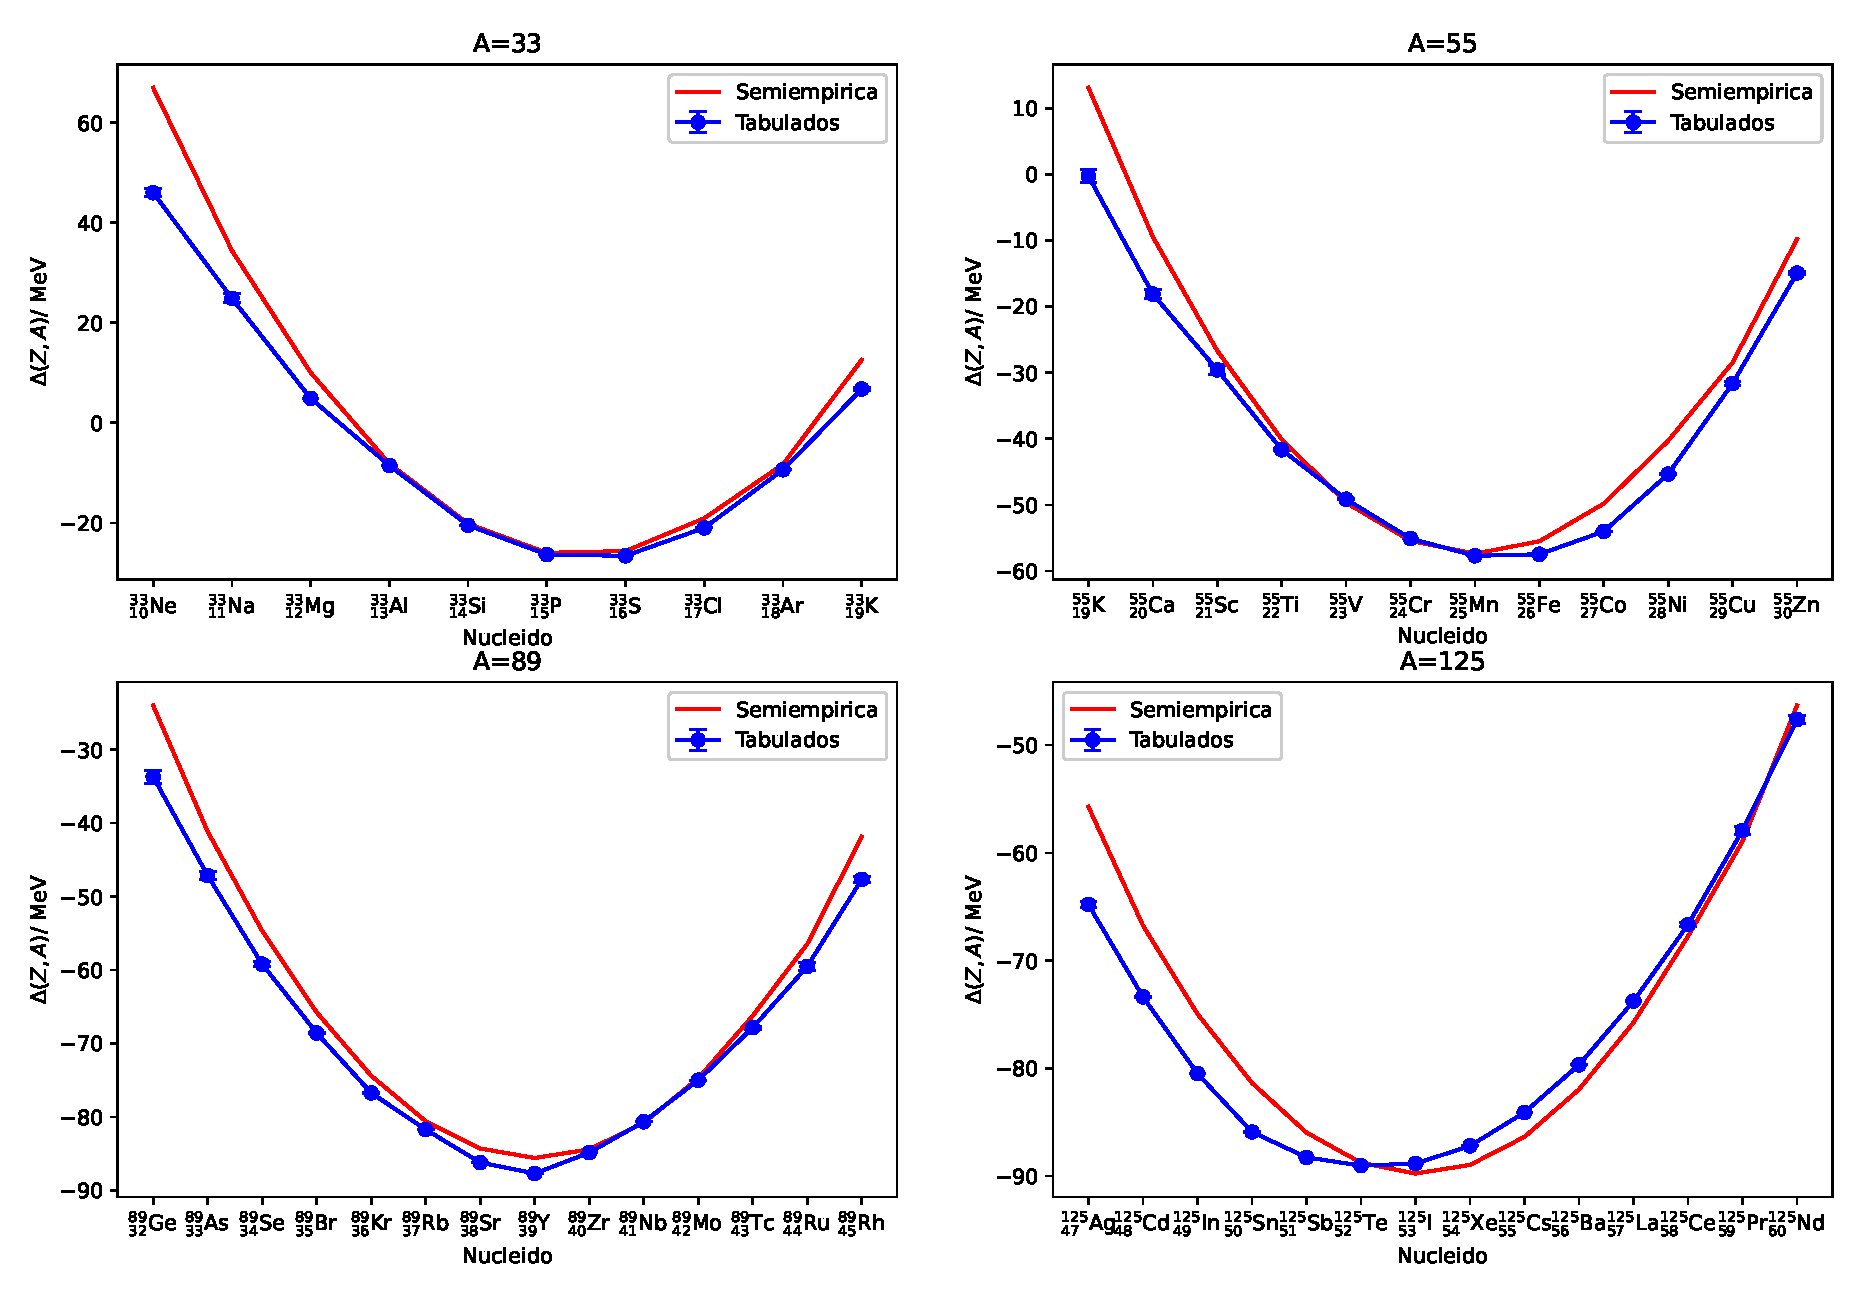
\includegraphics[width=\textwidth]{Imagenes/Parabola_masas.eps}
	 \caption{Valores dados por la semiempírica vs valores tabulados. Como podemos comprobar los valores tabulados son mejores cuanto más estables son los núcleos y más pequeños son.}
\end{figure}
Para $A$ constante, la masa atómica dada por la fórmula semiempírica de masas es una función cuadrática de $Z$: una parábola. En efecto, reuniendo los términos que acompañan a cada potencia de $Z$ tenemos que:

\begin{equation}
	\begin{split}
	M(Z,A)c^2  = \ & \ \parentesis{Am_n c^2 - a_v A + a_s A^{2/3} +a_{sy} A - \delta (A)} \\
	 + \ & \ \parentesis{m_p c^2 + m_e c^2 - m_n c^2 - a_c A^{-1/3} - a_cA^{-1/3} - 4a}Z \\
	 + \ & \ \parentesis{a_c A^{-1/3}+4a_{sy}A^{-1}}Z
	\end{split}
\end{equation}
donde hay que recordar que $M(Z,A)$ es la masa del núcleo, y en general $M(\ce{^1H})=m_p+m_e$. Derivando para encontrar el mínimo

\begin{eqnarray}
	Z_{\min} = \frac{\ccorchetes{m_n - m_p}c^2 + a_c A^{-1/3}+4a_{sy}}{2a_c A^{-1/3} + 8 a_{sy} A^{-1}} \approx \frac{A}{2} \parentesis{1+\frac{A^{2/3}a_c}{4a_{sy}}}^{-1}
\end{eqnarray}
Para los términos de $A$ par, el término \textit{pairing} ($\delta$) produce dos parábolas desplazadas una de la otra por $2\delta$. 


\section{Abundancia y estabilidad nuclear}

Si graficamos el número atómico $Z$ en función del número neutrónico $N$ (\textbf{carta de Segré}), observamos que los núcleos estables se acumulan en una banda estrecha alrededor de la línea $Z=N$ ($N/Z\approx 1$) hasta $A\approx 40$, mientras que a partir de $Z=80$ tenemos que $N/Z\approx 1.5$.

La abundancia relativa de los elementos en el Sistema solar no se deduce únicamente de los criterios de estabilidad, esta abundancia viene determinada más bien a partir de las características de las reacciones de nucleosíntesis en una época temprana del Universo. 

\begin{figure}[h!] \centering
	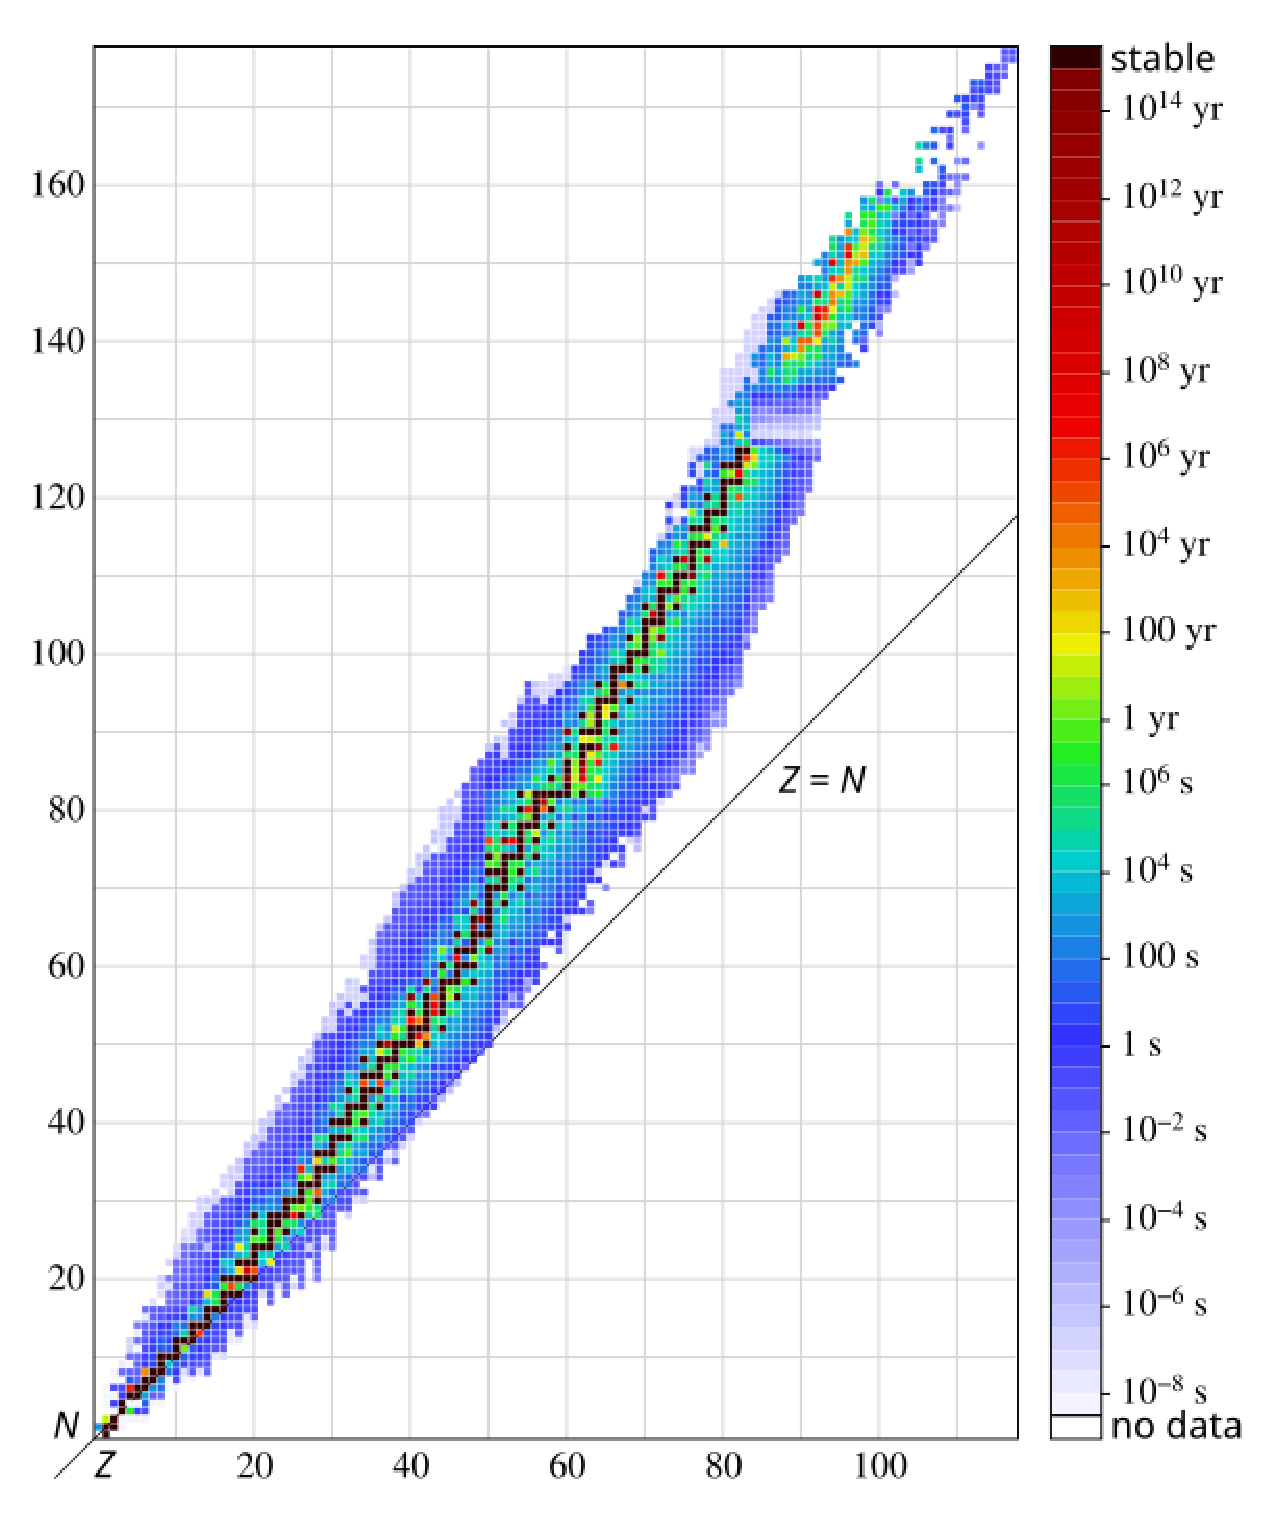
\includegraphics[width=0.5\textwidth]{Imagenes/Half-life.eps}
	\caption{Estabilidad de los diferentes nucleidos.}
\end{figure}


\section{Tamaño de los núcleos}

\subsection{Introducción}

El tamaño de los núcleos atómicos es del orden de unos cuantos fermis. Una manera de determinar el tamaño de los núcleos consiste en hacer dispersión de electrones sobre ellos. Esto permitiría estudiar la distribución de carga 

\subsection{Sección eficaz diferencial y sección eficaz total}

En los cursos introductorios de física cuántica se estudia la dispersión o colisión de partículas por potenciales simples en una dimensión. Este tratamiento sencillo es suficiente para ilustrar los conceptos de trasmisión y reflexión de partículas, efecto túnel, etc. En el caso de un potencial unidimensional la partícula incidente solo tiene dos posibilidades: seguir hacia delante o rebotar hacia atrás, cada una con cierta probabilidad (asumiendo que los potenciales son incapaces de mantener estados ligados). En tres dimensiones tendremos que considerar todo el continuo posible de direcciones emergentes de la partícula inicial tras la colisión. En el caso de colisiones profundamente ineslásticas surge además la complicación adicional de que se pueden crear más partículas en el estado final.

La manera más adecuada de describir la distribución angular de las partículas dispersadas por un centro de fuerzas o potencial se realiza mediante la denominada \textbf{sección eficaz}. Veremos que esta distribución angular proporciona importante información sobre el potencial dispersor, y, por tanto, sobre la partícula o sistema que lo crea.

Supongamos un haz incidente que transporta $N$ partículas por unidad de área y por unidad de tiempo (es un flujo, que se puede denotar por $\Phi$), y que lo hacemos incidir sobre un blanco que contiene $n$ centros dispersores. Si suponemos que el flujo incidente no es tan intenso como para provocar interferencia entre las propias partículas incidentes, que te tiene lugar una sola dispersión por partícula o que no hay una disminución apreciable de los centros dispersores del blanco por el retroceso de la partícula golpeada, entones el número de partículas incidentes que emergen por unidad de tiempo en un pequeño intervalo de ángulo sólido $\Delta \Omega$ centrado en los ángulos $\theta$ y $\phi$ será proporcional a $N,n$ y $\Delta \Omega$:

\begin{equation}
	\Delta \Ncal \sim n N \Delta \Omega
\end{equation}
Denotando por $\sigma (\theta, \phi)$ la constante de proporcionalidad, podemos escribir ese número de partículas emergentes en $\Delta \Omega$ por unidad de tiempo como:

\begin{equation}
	\Delta \Ncal = n N \sigma (\theta,\phi) \Delta \Omega
\end{equation}
o en intervalo diferencial

\begin{equation}
	\D \Ncal = n N \sigma (\theta,\phi) \D \Omega
\end{equation}
A la constante de proporcionalidad $\sigma(\theta,\phi)$ se le denomina \textbf{sección eficaz diferencial} y, como se puede ver a partir de la ecuación anterior, tiene unidades de área. En efecto $\sigma (\theta,\phi)\D \Omega$ es igual al área transversal del haz incidente paralelo que contiene el número de partículas dispersadas $\D \Omega$ por un único centro dispersor  o partícula del blanco. Evidentemente, a la integral de esa sección eficaz diferencial sobre la esfera se le denomina \textbf{sección eficaz total}

\begin{equation}
	\sigma_t = \int \sigma (\theta,\phi) \D \Omega
\end{equation}
En caso de dispersión sobre un blanco fijo la definición anterior de sección eficaz es igualmente válida para el sistema laboratorio \footnote{Recordemos que el sistema de referencia laboratorio es aquel en el que la partícula blanco está inicialmente en reposo mientras que el sistema de referencia centro de masas es aquel en el que el centro de masas está (siempre) en reposo.} que para el sistema centro de masas, porque un centro dispersor fijo tiene masa efectiva infinita. Para el caso de una colisión entre partículas de masa finita la definición anterior es en general válida sólo para el sistema de referencia laboratorio, y para la observación de la dispersión de la partícula incidente. No describe la dispersión angular del retroceso de la partícula bombardeada, aunque es por supuesto posible obtenerla a partir de la sección eficaz de la partícula incidente. La definición de la sección eficaz diferencial en el sistema del centro de masas puede hacerse de modo completamente análogo al anterior donde, de nuevo, lo que se observa es la dispersión de las partículas incidentes, pero el flujo incidente tiene que calcularse respecto a las partículas bombardeadas, no respecto al centro de masas. Como en el sistema centro de masas las dos partículas interaccionantes se mueven en sentidos opuestos después de la colisión, la sección eficaz diferencial para la observación del retroceso de la partícula blanco es simplemente $\sigma_{\textbf{blanco}} = \sigma_{\textbf{haz}} (\pi - \theta, \phi+\pi)$, ($\theta$ y $\phi$ referidos al centro de masas).

En general, la probabilidad de interacción de dos partículas depende fuertemente de la energía \footnote{Por ejemplo, la sección eficaz de captura de neutros térmicos por parte del uranio varía varios ordenes de magnitud en un pequeño rango de energía.}. La sección eficaz diferencial también se suele expresar en el intervalo diferencial de energía, de modo que para obtener la sección eficaz total habrá que integrar a todo rango de energías accesibles.

\begin{equation}
	\sigma_t = \iint\sigma(\theta,\phi) \D \Omega \D E
\end{equation}
La sección eficaz total es la suma de las dos partes: la sección eficaz inelástica\footnote{Más sobre esto en el tema de reacciones nucleares \ref{Ch:03}}:

\begin{eqnarray}
	\sigma_{\tot} = \sigma_{\el}+ \sigma_{\inel}
\end{eqnarray}
La unidad comúnmente usada para las secciones eficaces es el barn

\begin{eqnarray}
	1 \unit{barn} = 10^{-24} \ \unit{\cm^{2}} = 10^{-28} \  \unit{\m^2} = 100 \ \unit{\fm^2}
\end{eqnarray}


\subsection{Sección eficaz de Rutherford}

La sección eficaz para la dispersión elástica coulombiana de partículas puntuales sin espín se conoce como la sección eficaz de Rutherford. Él fue el pionero en el uso de las técnicas de dispersión para el estudio del mundo subatómico, concretamente bombardeanddo una lámina de oro con partículas $\alpha$. Supongamos ahora una colisión elástica entre un electrón y un núcleo en reposo de carga $Ze$. Despreciemos por el momento efectos de espín y supongamos además que el electrón se aproxima en trayectoria hiberbólica con velocidad no relativista $v$ y que la energía de retroceso del nucleo es despreciable frente a la interacción. Usando mecánica clásica no relativista es sencillo derivar la siguiente expresión para la sección eficaz diferencial de Rutherford:

\begin{equation}
	\parentesis{\derivadas{\sigma(\theta)}{\Omega}}_{\text{Rutherford}} = \parentesis{\frac{Ze^2}{8 \pi \epsilon_0 m_e v^2}}^2 \frac{1}{\sin^4 (\theta/2)} = \parentesis{\frac{Ze^2}{ 4 \pi \epsilon_0}}^2 \frac{1}{(4E)^2\sin^4 (\theta/2)}
\end{equation}
donde $E=mv^2/2$ es la energía cinética del electrón y $\theta$ el ángulo polar de dispersión. Si la energía de retroceso del núcleo no fuera despreciable, entonces deberíamos sustituir la expresión anterior de $m_e$ por la masa reducida $\mu=m_em_N / (m_e+m_N)$, $v$ sería la velocidad del centro de masas y el ángulo de dispersión $\theta$ estaría referido al sistema de referencia del centro de masas.

La mecánica clásica es una teoría completamente determinista, de tal modo que dadas unas ciertas condiciones iniciales es posible predecir exactamente la trayectoria de la partícula y, por tanto, el diferencial de ángulo sólido por el que pasará una vez dispersada. Si imaginamos un haz uniforme de partículas con cierta sección transversal incidiendo sobre una lamina de material a modo de blanco, la ecuación anterior nos da la proporción de partículas que en la unidad de tiempo saldrán dispersadas atravesando una superficie diferencial perpendicular a $\D \Omega$. En este problema el campo de fuerzas es central, de modo que existe simetría azimutal y podemos integrar sobre el ángulo $\phi$ para obtener:

\begin{equation}
	\D \Omega = \int_0^{2\pi} \sin (\theta) \D \theta \D \phi = 2 \pi \sin (\theta) \D \theta
\end{equation}
por eso escribimos directamente $\sigma = \sigma (\theta)$.

La sección eficaz de Rutherford es una de las pocas fórmulas de la mecánica clásica que también se deduce en el formalismo de la mecánica cuántica. Pero en el \textit{mundo cuántico} su significado es distinta: representa la probabilidad de que una partícula salga dispersada en un ángulo sólido diferencial $\D \Omega$, aunque también es cierto que en el caso de un haz de partículas incidiendo sobre el blanco representa una fracción de ellas que en la unidad de tiempo atravesarán una superficie diferencial a $\D \Omega$, al igual que en el caso clásico.

Una manera rápida de deducir la sección eficaz de Rutherford en mecánica cuántica es mediante la primera aproximación de Born. Se considera que la función de onda inicial y final del electrón está bien descrita por una onda plana, tal que $\pn_i=\hbar \kn_i$ y $\pn_f = \hbar \kn_f$ (donde $|k|=2\pi / \lambda$).  En ese caso las funciones de onda inicial y final

\begin{equation}
	\Psi_i (\rn) \sim e^{i \pn_i \cdot \rn / \hbar} \tquad \Psi_f (\rn) \sim e^{i \pn_f \cdot \rn / \hbar}
\end{equation}
El potencial $V(\rn)$ del centro dispersor \textit{convierte} la onda plana inicial en la onda plana final, y la amplitud de probabilidad de la transición viene dada, en primera aproximación de Born Por
\begin{equation}
	f(\pn_i,\pn_f) \sim \int \Psi_f^* V \Psi_i \D^3 \rn \sim \int e^{i \qn \cdot \rn / \hbar} V(\rn) \D^3 \rn \sim f(\qn)
\end{equation}
donde $\qn=\pn_i - \pn_f$ es el \textbf{momento trasnferido en la colisión}. La sección eficaz diferencial es el módulo al cuadrado de esta \textit{amplitud de probabildiad}

\begin{equation}
	\frac{\D \sigma}{\D \Omega} = | f(\qn) |^2
\end{equation}
Por lo que si el potencial es simétrico $V(\rn)=V(r)$, podemos integrar sobre los ángulos y obtener:

\begin{equation}
	f(\qn) \sim \int_0^\infty r V(r) \sin (qr/\hbar) \D r
\end{equation}
Si escribimos $V(r)=-Ze^2/4\pi \epsilon_0 r$ la integral anterior no existe (se va a infinito). Sin embargo $V(r)$ no tiene dicha forma, ya que en realidad la carga del núcleo $Ze$ está apantallada por la carga electrónica, de tal manera que a grandes distancias la partícula incidente no \textit{ve} el potencial eléctrico desnudo del núcleo. Se puede tener en cuenta este apantallamiento añadiendo un factor multiplicativo exponencial

\begin{equation}
    V(r) =  - \frac{1}{4 \pi \epsilon_0} \frac{Ze^2}{r} e^{-r/a}
\end{equation}
donde $a$ es una longitud característica de las dimensiones atómicas. La integral sobre el radio produce entonces el siguiente resultado

\begin{equation}
    f(\qn^2) \sim \frac{Ze^2}{q^2+(\hbar/a)^2} \approx \frac{Ze^2}{q^2}
\end{equation}
Finalmente, si reunimos todas las constantes que no hemos ido poniendo explícitamente la sección eficaz puede escribirse como:

\begin{eqnarray}
	\derivadas{\sigma}{\Omega} = \frac{4Z^2\alpha^2 (\hbar c)^2 E^2 }{|\qn c|^4}
\end{eqnarray}
donde $\alpha = e^2 / 4 \pi \epsilon_0 \hbar c$ es la \textit{constante de estructura fina}. Para comprobar que esta fórmula coincide con la primera que hemos dado basta con observar que en una colisión elástica en la que se desprecia el retroceso se cumple que $|\pn_i|=|\pn_f|=|\pn|$ y por tanto el módulo de $\qn$ ($\qn=\pn_i-\pn_f$)

\begin{eqnarray}
	|\qn|^2 = 4 p^2 \sin^2 (\theta/2) \ \rightarrow \ q = 2p \sin (\theta/2)
\end{eqnarray}
Siempre que tomemos el límite no relativista ($E=\sqrt{p^2c^2+c^4m^2}\approx mc^2$) podremos deducir la primera ecuación. Uno de los problemas del cálculo de esta ecuación es que hemos asumido que la partícula incidente y la partícula blanco tienen espín cero, lo cual no es verdad. Además es que tampoco es despreciable cuando hablamos de dispersión de electrones, ya que las energías son tan altas que debemos tener en cuenta los efectos del espín del electrón. La \textbf{sección eficaz de Mott} describe la dispersión relativista de electrones, incluyendo efectos de espín, sobre partículas puntuales sin espín:

\begin{eqnarray}
	\parentesis{\derivadas{\sigma(\theta)}{\Omega}}_{\text{Mott}}^* = 
	\parentesis{\derivadas{\sigma(\theta)}{\Omega}}_{\text{Rutherford}} \ccorchetes{1-\beta ^2 \sin^2(\theta/2)} 
\end{eqnarray}
donde $\beta=v/c$.





\subsection{Factor de forma}

Consideremos entonces que el núcleo atómico es un objeto extenso con una densidad de carga eléctrica que podamos expresar en la forma $Ze\rho (\rn')$, de tal manera que $\rho(\pn')$ es una densidad de probabilidad normalizada $\int \rho (\rn') \D^3 (\rn')=1$. Si además la distribución de carga fuese esféricamente simétrica tendríamos

\begin{equation}
	4 \pi \int_0^\infty \rho (r) r^2 \D r = 1
\end{equation}

% Faltan coas

La integral restante en la expresión de $f(\qn)$ se conoce como \textbf{factor de forma}

\begin{equation}
    F(\qn) = \int \rho (\rn) e^{i \qn \cdot \rn / \hbar} \D^3 \rn
\end{equation}
En el caso de que tratemos distribuciones eféricamente simétricas, el factor de forma sólo dependerá del cuadrado del momento transferido.
\begin{equation}
    F(\qn^2) = \int \rho (r) e^{i \qn \cdot \rn / \hbar} \D^3 \rn
\end{equation}
Recordando que $\D \sigma / \D \Omega = |f|^2$ tenemos que

\begin{equation}
    \parentesis{\derivadas{\sigma}{\Omega}}_{\text{extenso}} = \parentesis{\derivadas{\sigma}{\Omega}}_{\text{Ruth.}} \cdot |F(\qn^2)|^2
\end{equation} 
donde la etiqueta \textit{extenso} hace referencia a que hemos considero al núcleo como un objeto extenso y no como una partícula puntual. Vemos por lo tanto que la sección eficaz de dispersión por un centro extenso de carga es igual a la sección eficaz de dispersión por un centro puntual multiplicada por el cuadrado del factor de forma. Toda la información sobre la extensión espacial del núcleo reside en su factor de forma, que no es otra cosa que la transformada de Fourier de la distribución de carga. En el caso de la dispersión de electrones tenemos que usar la dispersión de Mott:

\begin{equation}
	\parentesis{\derivadas{\sigma}{\Omega}}_{\text{extenso}} = \parentesis{\derivadas{\sigma}{\Omega}}_{\text{Mott}} \cdot |F(\qn^2)|^2
\end{equation} 

Para pasar de $F(\qn^2)$ a la distribución de carga $\rho(r)$ podríamos pensar, en principio, en invertir la ecuación del factor de forma:

\begin{equation}
    \rho(r)=\frac{1}{(2\pi)^3} \int F(\qn^2) e^{-i \qn \cdot \rn/\hbar} \D^3 q
\end{equation}
Esta ecuación nos permite obtener $\rho(r)$ si antes hemos medido $F(\qn^2)$ para todos los valores de $\qn^2$. No obstante, el rango del momento transferido está limitado experimentalmente por los máximos momentos disponibles para las partículas haz. Además la sección eficaz es muy pequeña para valores grandes de $\qn^2$. 

\subsection{Ejemplos de factores de forma}

Las primeras medidas de factores de forma nucleares fueron llevados a cabo a principios de la década de los 50 en SLAC\footnote{Standford Lineal Accelerator.}. Se midieron secciones eficaces para una gran variedad de núcleos con electrones de energía hasta 500 MeV. Los resultados muestran un rápido decrecimiento de la sección eficaz para grandes ángulos, que se corresponde con el hecho de que la dependencia con el momento transferido va como $1/\qn^4$, (recuérdese que $|\qn|=2|\pn| \sin (\theta /2)$). Para distribuciones simñetricas de carga podemos integrar sobre el ángulo sólido y obtener:

\begin{equation}
	F(\qn^2) = 4 \pi \int \rho (r) \frac{\sin (|\qn|r/\hbar)}{ |\qn| r / \hbar} r^2 \D r
\end{equation}

Introduciendo en la expresión anterior distribuciones sencillas de carga de modo que podamos realizar la integral, obtendremos ejemplos de factores de forma a comparar con las mediciones y así hacernos una idea intuitiva de la distribución de carga nuclear. En las figuras tenemos varios ejemplos. Para una carga puntual (delta de Dirac) el factor de forma es una constante (la unidad). Cuanto más extesa sea la distribución espacial de carga más rapidamente decrecerá con $\qn$ el factor de forma. En el límtie de una distribución extendida por todo el espacio tendríamos una delta de Dirac para el factor de forma. Para una distribución gaussiana tendríamos otra distribución gaussiana. Para una esfera homogénea tendriamos osciliaciones típicas de un patrón de difracción con mínimos que se anulan. Para una esfera con superficie difusa tendríamos oscilacioens difuminadas, con mínimos que no llegan a anularse. \\

% faltan cosas

El valor medio del cuadrado del radio $\langle r^2 \rangle$ está dado por la fórmula

\begin{equation}
	\langle r^2 \rangle = \int r^2 \rho (r) \D \rn^3 = 4\pi \int r^2 \rho (r) r^2 \D r
\end{equation} equation
% Faltan pocas coasas

Se observa que los núcleos no tienen una superficie bien definida, sino más bien difusa. En su interior la distribución de carga es aproximadamente constante, y en la superficie decrece en un cierto rango hasta hacerse nula. Una buena parametrización de esta distribución se consigue con la llamada \textbf{función de Fermi de dos parámetros} también llamada \textbf{distribución de Wood-Saxon}:

\begin{equation}
    \rho (r) = \frac{\rho(0)}{1+e^{(r-c)/a}}
\end{equation}
donde $c$ es el radio al que $\rho(r)$ decrece a la mitad del valor del plató \footnote{Caamaño llama a la constante $R_{1/2}\equiv c$}.
\begin{figure}[h!]  \centering
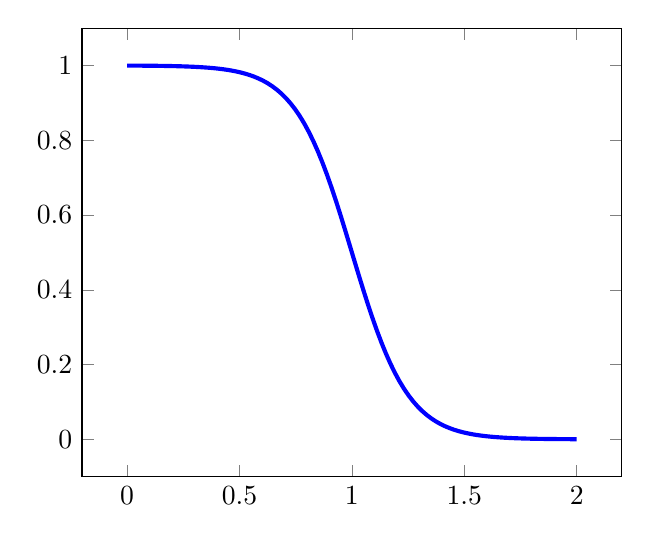
\begin{tikzpicture}
	\begin{axis}
		\addplot+ [
		domain=0:2,
		samples=100, 
		mark=none, % Esto elimina los puntos
	 	line width=1.5pt % Aumenta el grosor de la línea 
	%	thick 	
		] {1/(1+exp(8*(x-1))};
	\end{axis}
\end{tikzpicture}
\caption{Potencial Wood-Saxon ($c=1$, $a=1/8$).}
\end{figure}


El parámetro $a$ está relacionado con el grosor de la piel \footnote{$t$ es la distancia que necesita la densidad de carga para caer del $90\%$ al $10\%$ de su valor} (skin thickness) mediante $t=(4\ln 3)a$. Los resultados experimentales indican para núcleos pesados y medios se cumplen 

\begin{equation}
	\sqrt{\langle r^2 \rangle} = r_0 A^{1/3} \tquad r_0 = 0.94 \unit{\fm}
\end{equation}



El volumen nuclear es, por lo tanto, proporcional al número de nucleones $A$, y la densidad de carga nuclear es aproximadamente constante (comportamiento similar a líquidos o sólidos). El radio a mitad de densidad y el grosor de la piel satisfacen, aproximadamente, la siguiente relación:

\begin{equation}
    c(\unit{\fm}) = 1.18A^{1/3} - 0.48 \tquad t \approx 2.4 \unit{\fm}
\end{equation} \\

% Faltan cosas
También se suele utilizar la \textbf{función de Fermi de tres parámetros} que se define como

\begin{equation}
    \rho (r) = \parentesis{1+ \frac{\omega r^2}{c^2}} \frac{\rho (0)}{1+e^{(r-c)/a}} 
\end{equation}
Se puede determinar la distribución de carga a partir de los datos experimentales con un método casi independiente del modelo si la escribimos como una superposición de gaussianas:

\begin{equation}
	\rho (r) \propto \sum_{i=1}^N A_i \exp \ccorchetes{- \frac{(r-R_i)^2}{\delta_i}}
\end{equation}
Es preciso tener en cuenta, sin embargo, que la dispersión de electrones proporciona información sobre la distribución de carga eléctrica, pero para investigar la distribución de materia nuclear necesitamos proyectiles hadrónicos.

